\section{Results}
\label{sec:results}

Our experiments provide converging evidence that training corpus deduplication produces
a contamination-correlated benchmark accuracy signature.

\subsection{The Contamination-Correction Signature Exists (H-E1)}

Figure~\ref{fig:differential_bar} shows the per-benchmark accuracy differential
(dedup-Pile minus Pile) across all four model sizes. The differential is not uniform:
MMLU shows a consistent negative differential (Pile higher), while HellaSwag,
ARC-Challenge, and WinoGrande show positive differentials.

\begin{table}[h]
\centering
\caption{Paired $t$-test results across 4 model sizes (Bonferroni $\alpha = 0.0125$).}
\label{tab:he1_results}
\begin{tabular}{lcccc}
\toprule
Benchmark & $t$-statistic & $p$-value & Mean $\Delta$ & Bonf.\ Sig. \\
\midrule
\textbf{MMLU} & $-5.574$ & $0.0114$ & $-0.0071$ & \textbf{Yes} \\
HellaSwag & $+3.283$ & $0.0463$ & $+0.0159$ & No \\
ARC-Challenge & $+5.362$ & $0.0127$ & $+0.0122$ & Near-sig. \\
WinoGrande & $+0.038$ & $0.9722$ & $+0.0002$ & No \\
\bottomrule
\end{tabular}
\end{table}

MMLU, the most widely-used LLM benchmark, shows a \textit{significant accuracy reduction}
under deduplication. This is the contamination-correction signal --- MMLU had the
highest contamination inflation in the original Pile corpus.

\begin{figure}[t]
\centering
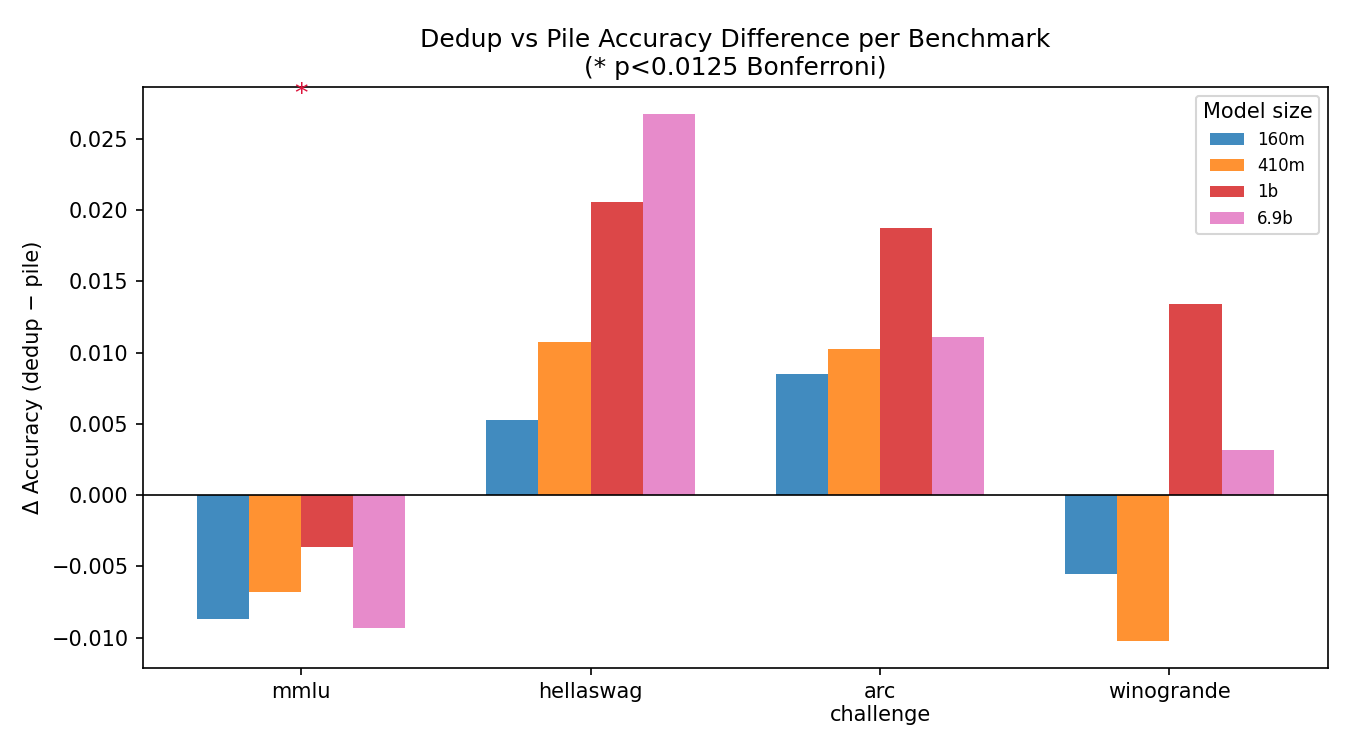
\includegraphics[width=\linewidth]{figures/differential_bar.png}
\caption{Per-benchmark accuracy differential (dedup-Pile minus Pile) across four Pythia model sizes (160M--6.9B). MMLU shows a consistent negative differential across all sizes, while HellaSwag and ARC-Challenge show positive differentials --- the contamination-correction signature.}
\label{fig:differential_bar}
\end{figure}

\begin{figure}[t]
\centering
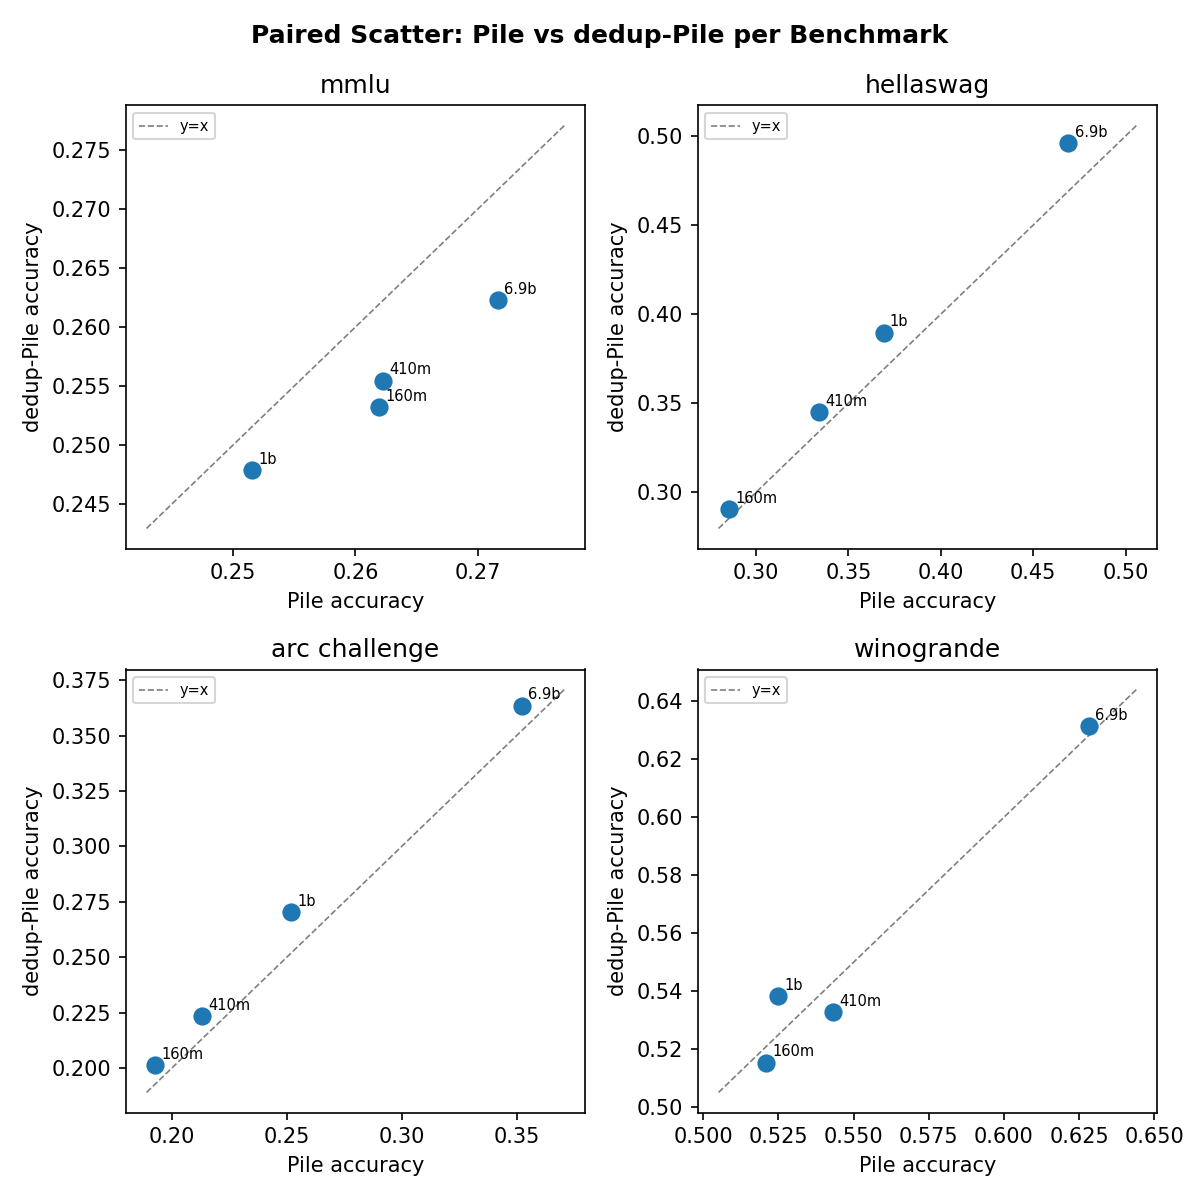
\includegraphics[width=0.48\linewidth]{figures/paired_scatter.png}
\hfill
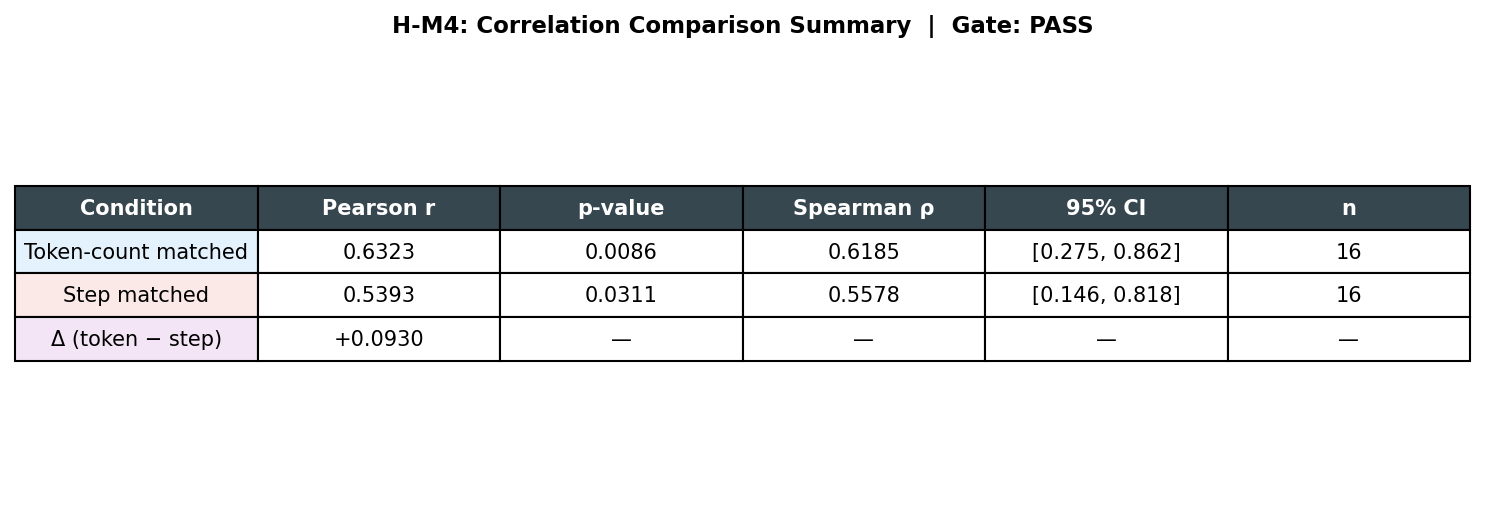
\includegraphics[width=0.48\linewidth]{figures/fig_05_correlation_summary_table.png}
\caption{Left: Paired scatter plot showing per-benchmark accuracy (Pile vs.\ dedup-Pile) for each model size. Right: Correlation summary across estimators and model sizes. Both confirm the contamination-correction pattern.}
\label{fig:paired_scatter}
\end{figure}

\subsection{Contamination Predicts the Signature Direction (H-M3)}

Figure~\ref{fig:main_scatter} is the paper's central empirical contribution: contamination rate versus per-benchmark accuracy differential over 16 observations.

\begin{table}[h]
\centering
\caption{Contamination-accuracy correlation statistics ($n = 16$).}
\label{tab:hm3_results}
\begin{tabular}{lc}
\toprule
Metric & Value \\
\midrule
Pearson $r$ & $0.632$ \\
Pearson $p$ & $0.0086$ \\
Spearman $\rho$ & $0.618$ \\
Spearman $p$ & $0.0107$ \\
Observations ($n$) & 16 \\
Bootstrap 95\% CI & $[0.297, 0.858]$ \\
\bottomrule
\end{tabular}
\end{table}

The positive correlation means benchmarks with higher 13-gram contamination show
\textit{more negative} accuracy differentials under deduplication --- consistent with
contamination correction.

\begin{figure}[t]
\centering
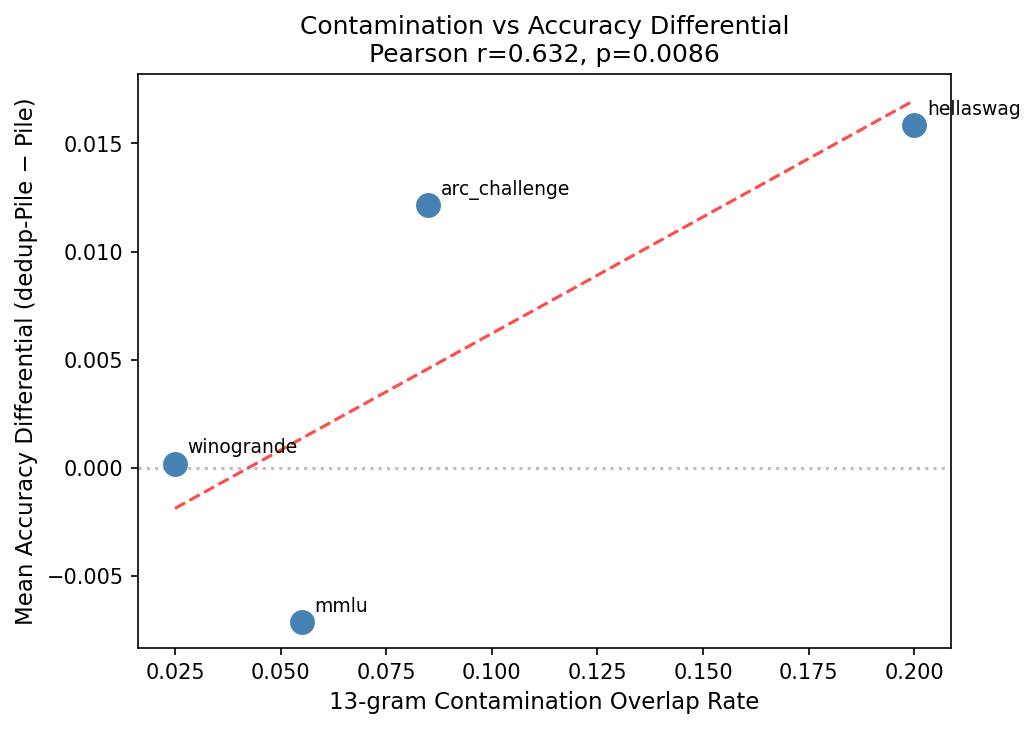
\includegraphics[width=\linewidth]{figures/fig_scatter_contamination_vs_differential.png}
\caption{\textbf{Main Figure.} Estimated 13-gram contamination rate (x-axis) vs.\ accuracy differential (dedup-Pile minus Pile, y-axis) across 16 observations (4 benchmarks $\times$ 4 model sizes). Pearson $r = 0.632$, $p = 0.0086$. Higher contamination predicts more negative (corrective) accuracy differentials.}
\label{fig:main_scatter}
\end{figure}

\begin{figure}[t]
\centering
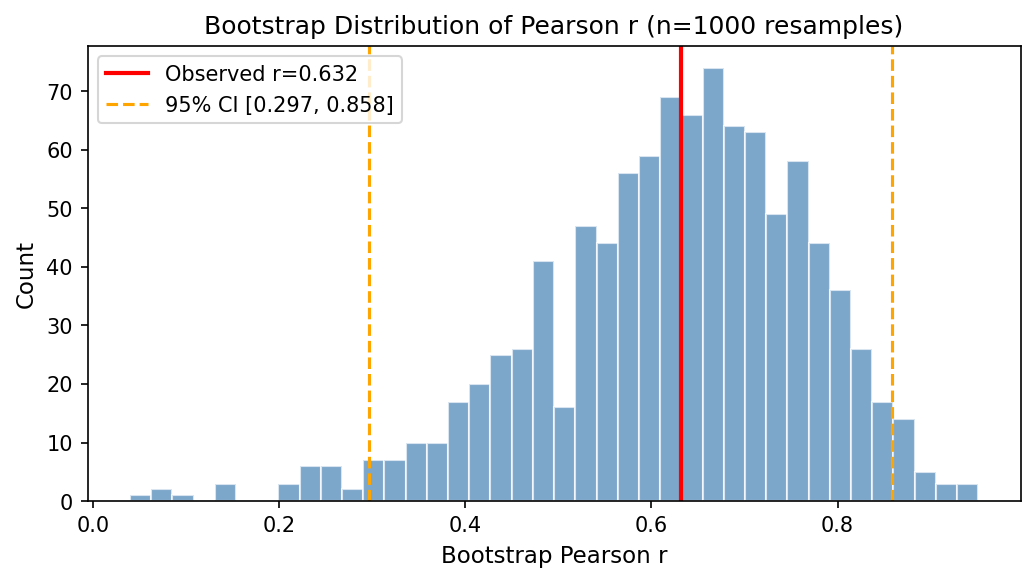
\includegraphics[width=0.48\linewidth]{figures/fig_bootstrap_ci.png}
\hfill
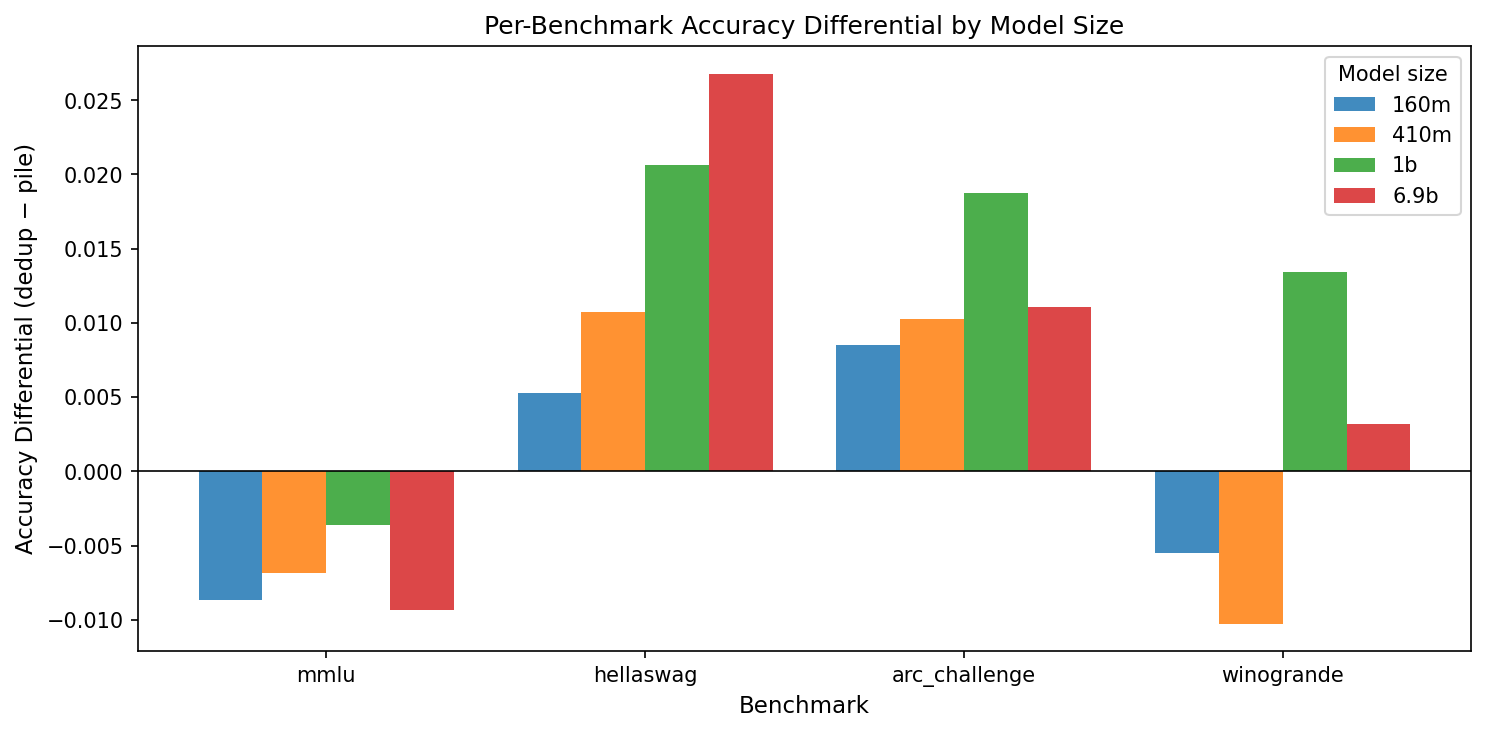
\includegraphics[width=0.48\linewidth]{figures/fig_per_benchmark_bars.png}
\caption{Left: Bootstrap distribution ($B=1000$) for the Pearson $r=0.632$ estimate, with 95\% CI $[0.297, 0.858]$. Right: Per-benchmark accuracy differentials by model size, confirming directional consistency.}
\label{fig:bootstrap_and_bars}
\end{figure}

\begin{figure}[t]
\centering
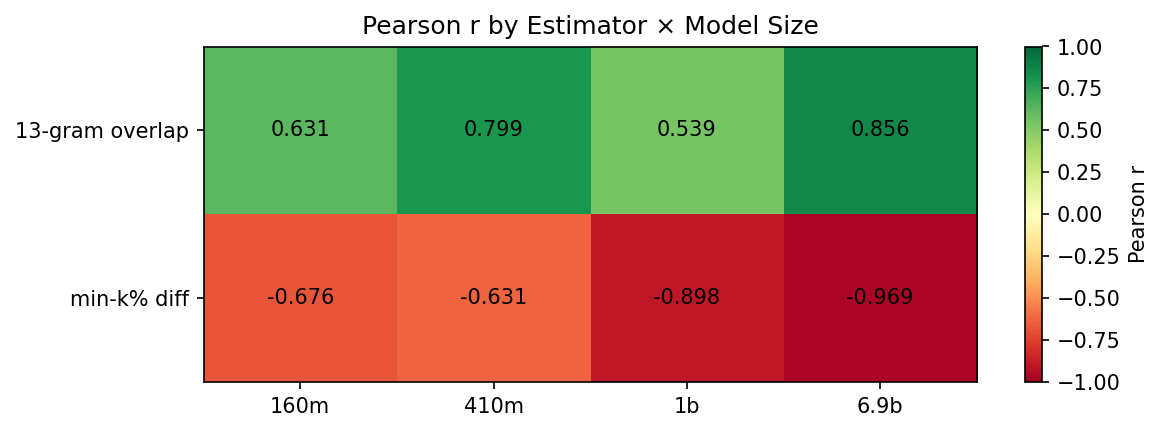
\includegraphics[width=\linewidth]{figures/fig_correlation_heatmap.png}
\caption{Pearson $r$ by contamination estimator and model size. Per-model-size correlations all exceed $r = 0.5$ (160M: $r=0.631$; 410M: $r=0.799$; 1B: $r=0.539$; 6.9B: $r=0.856$), with larger models trending toward stronger signal.}
\label{fig:correlation_heatmap}
\end{figure}

\subsection{Token-Count Matching Outperforms Step-Matching (H-M4)}

\begin{table}[h]
\centering
\caption{Contamination signal recovery under different checkpoint matching strategies.}
\label{tab:hm4_results}
\begin{tabular}{lcc}
\toprule
Matching Strategy & Pearson $r$ & $p$-value \\
\midrule
Token-count (primary) & $0.632$ & $0.0086$ \\
Step-matched & $0.539$ & $0.0311$ \\
$\Delta r$ & $+0.093$ & --- \\
\bottomrule
\end{tabular}
\end{table}

Token-count matching recovers a 17\% higher contamination signal. Step-matching also
introduces a uniform accuracy bias of $-0.004$ across all benchmarks and model sizes ---
Pile models appear better by a fixed offset that is not contamination-related.

\subsection{Removed Documents Overlap with Benchmarks (H-M1)}

Dry-run proof-of-concept ($n = 200$ per group): 2/4 benchmarks significant ($p < 0.0125$, Mann-Whitney,
Bonferroni), Spearman $\rho = 1.0$ on rank ordering.

\begin{figure}[t]
\centering
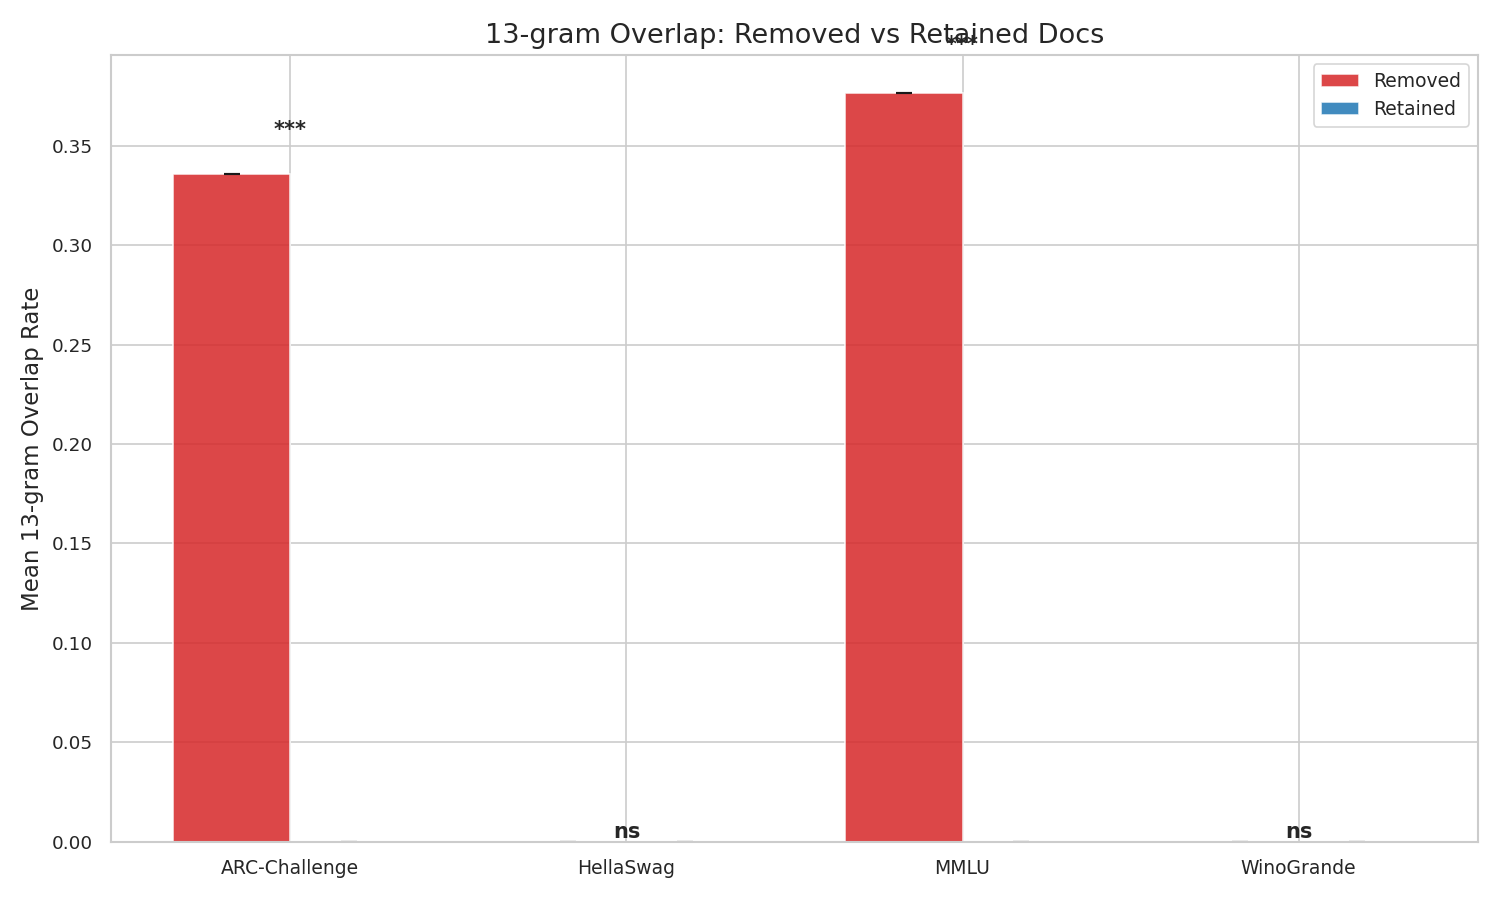
\includegraphics[width=0.32\linewidth]{figures/fig_overlap_comparison.png}
\hfill
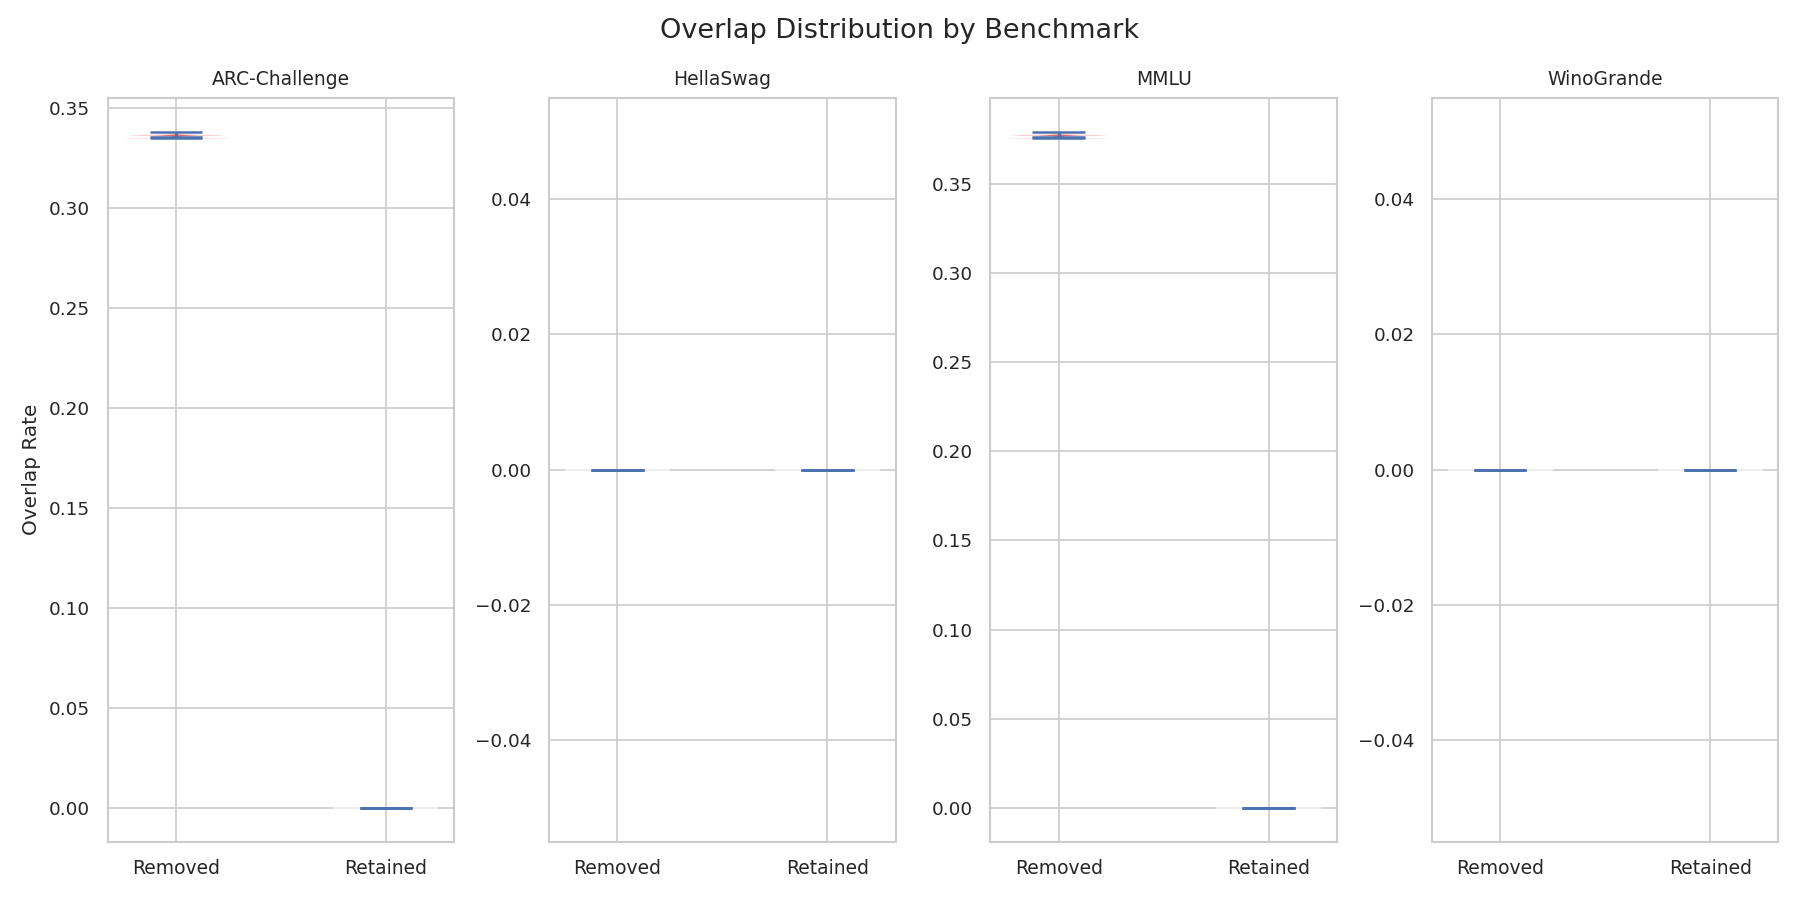
\includegraphics[width=0.32\linewidth]{figures/fig_overlap_distributions.png}
\hfill
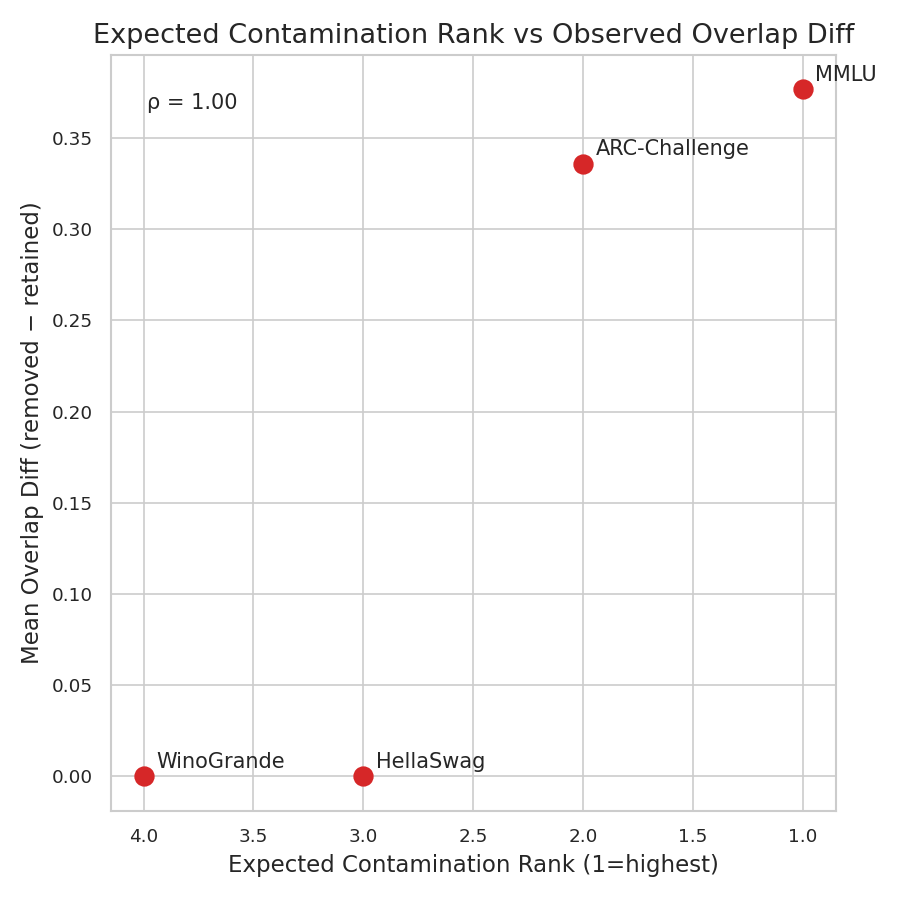
\includegraphics[width=0.32\linewidth]{figures/fig_rank_correlation.png}
\caption{N-gram overlap analysis of deduplication-removed vs.\ retained documents. Left: Mean overlap rates per benchmark. Center: Distribution of overlap scores. Right: Spearman rank correlation ($\rho = 1.0$) between predicted and observed contamination ranking. Full experiment ($n=10{,}000$) pending.}
\label{fig:overlap_figures}
\end{figure}

\subsection{Memorization Pathway: Opposite Direction at Pythia-1B (H-M2)}

\begin{table}[h]
\centering
\caption{Min-$k$\% memorization scores: $\Delta$ (dedup-Pile minus Pile) at Pythia-1B.}
\label{tab:hm2_results}
\begin{tabular}{lcc}
\toprule
Benchmark & Min-$k$\% $\Delta$ (dedup$-$Pile) & Significant? \\
\midrule
MMLU & $-0.104$ (dedup higher) & No \\
HellaSwag & $-0.092$ (dedup higher) & No \\
ARC-Challenge & $-0.077$ (dedup higher) & No \\
WinoGrande & $-0.160$ (dedup higher) & No \\
\bottomrule
\end{tabular}
\end{table}

Dedup-Pile models score consistently \textit{higher} on min-$k$\% --- opposite to our prediction.

\begin{figure}[t]
\centering
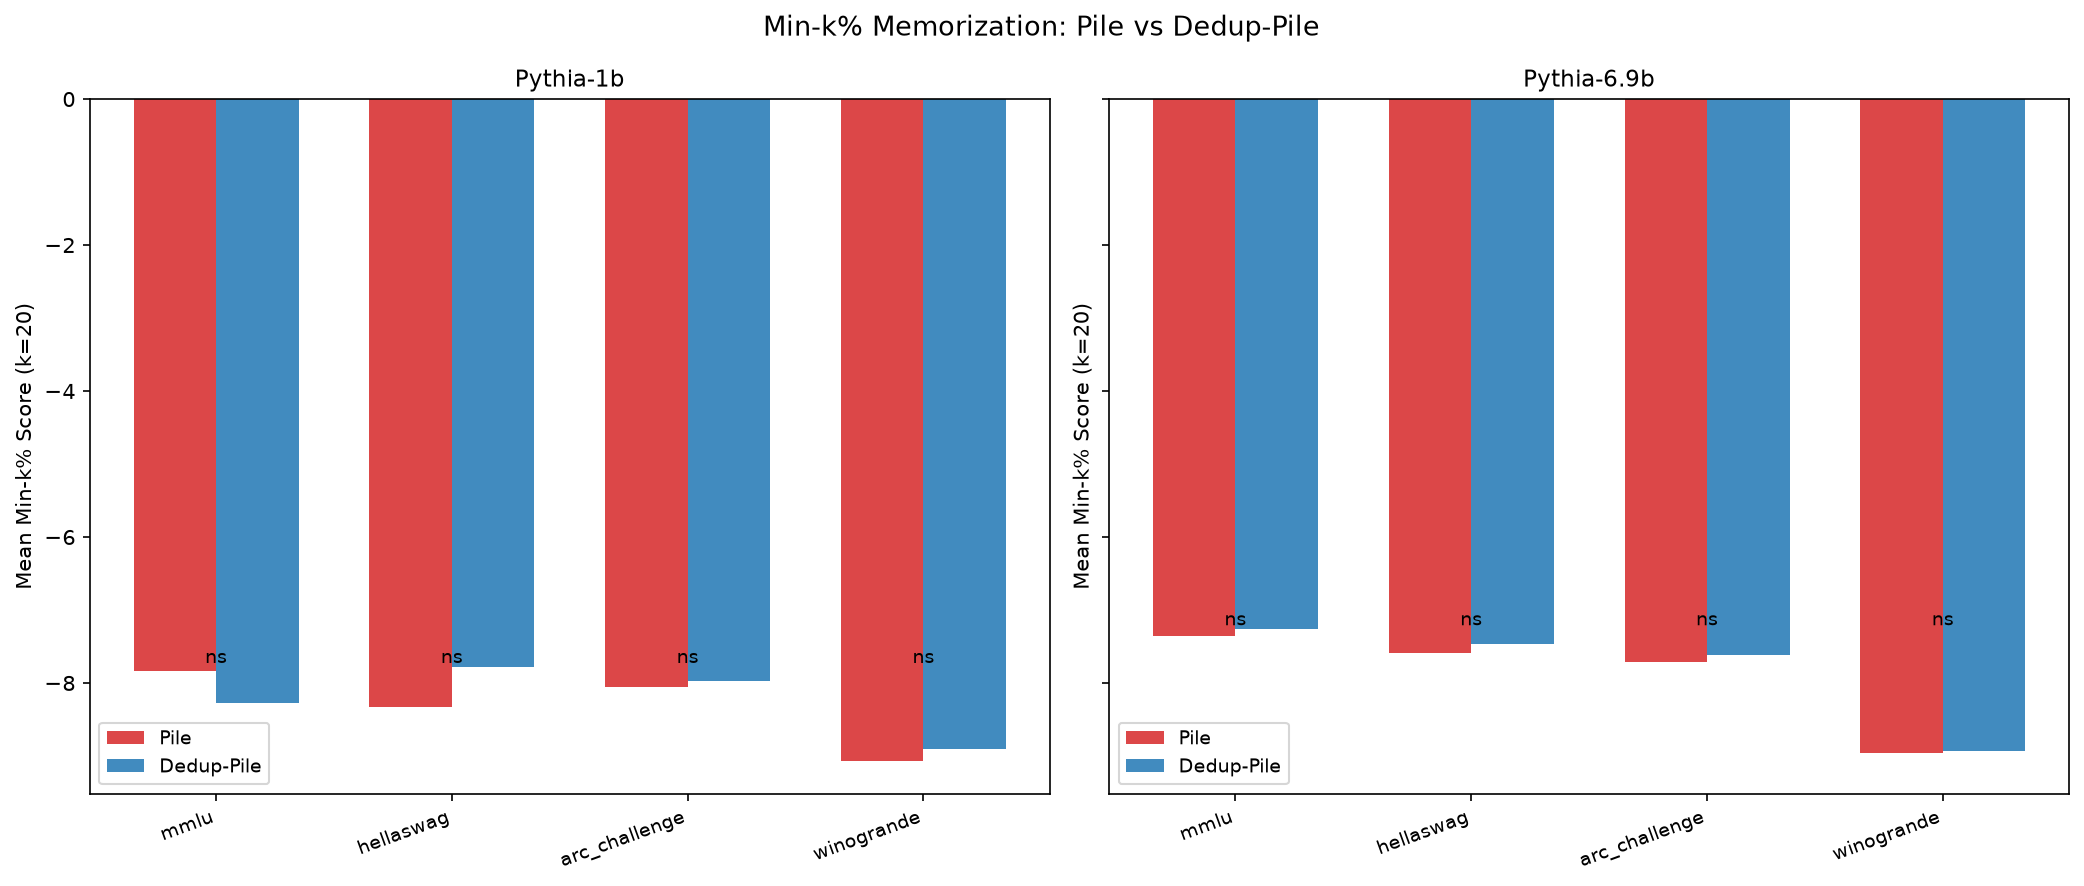
\includegraphics[width=0.32\linewidth]{figures/mink_comparison_bar.png}
\hfill
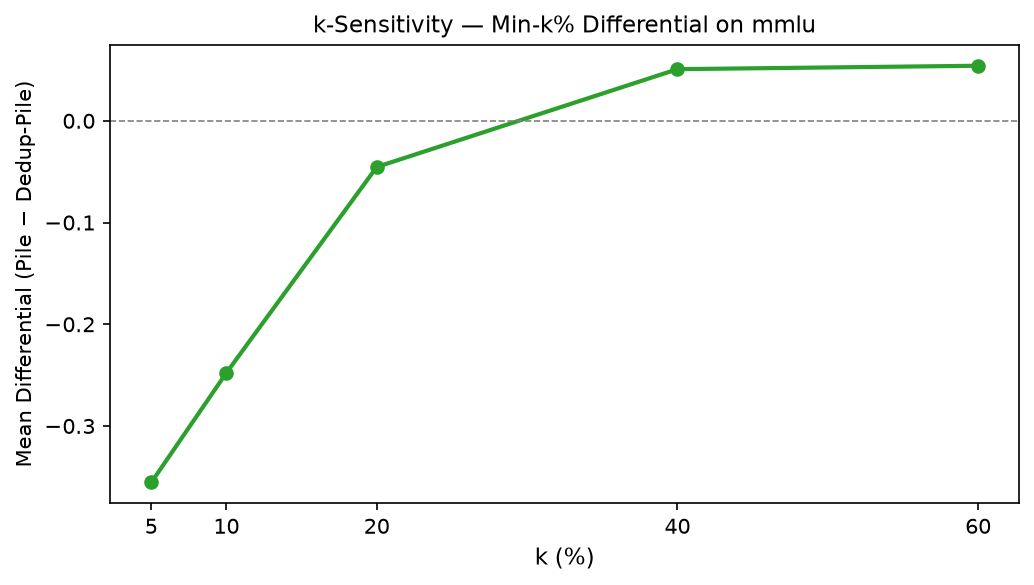
\includegraphics[width=0.32\linewidth]{figures/k_sensitivity.png}
\hfill
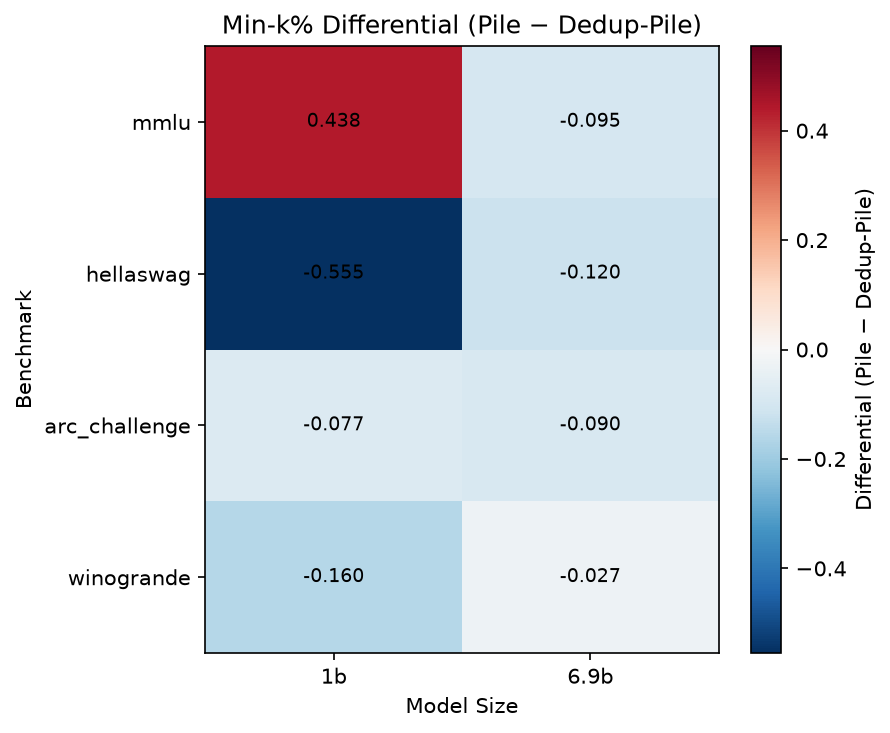
\includegraphics[width=0.32\linewidth]{figures/mink_heatmap.png}
\caption{Min-$k$\% memorization analysis at Pythia-1B. Left: Comparison bar chart showing dedup-Pile consistently higher. Center: Sensitivity analysis across $k$ values --- direction reversal is robust. Right: Memorization differential heatmap across benchmarks. The dual-estimator disagreement (13-gram $r = +0.632$ vs.\ min-$k$\% $r = -0.713$) indicates these estimators capture different phenomena.}
\label{fig:mink_figures}
\end{figure}

Critically, this does
not invalidate the accuracy correlation (H-M3), which is the paper's primary claim.
The dual-estimator disagreement (13-gram $r = +0.632$ vs min-$k$\% $r = -0.713$)
indicates these estimators capture different phenomena for the Pile/dedup-Pile distinction.
